\label{ex:EstimationOverNetwork}
\begin{figure}
  \begin{center}
    {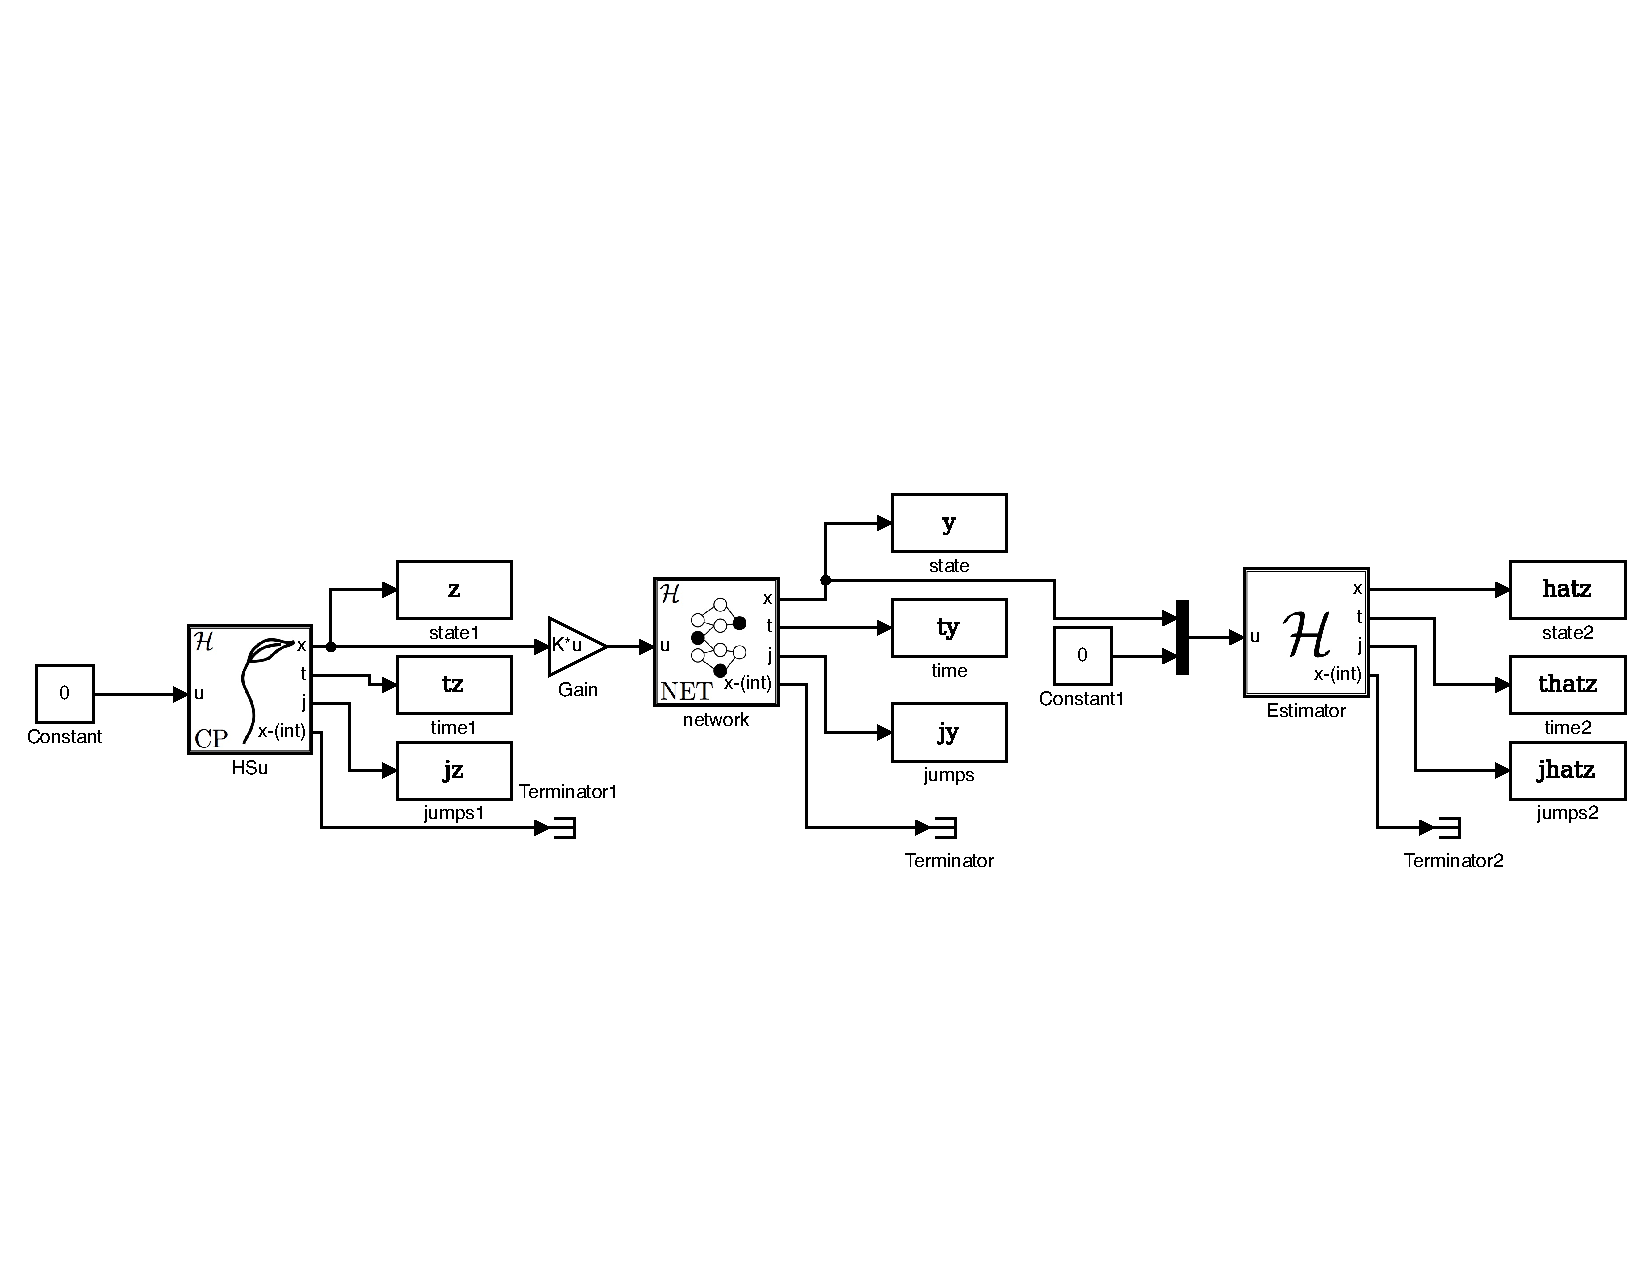
\includegraphics[width=1.0\textwidth]{figures/Simulink/NetworkExample.pdf}}
   \caption{Estimation over a network scheme in Example~\ref{ex:Estimation}.}
\label{fig:NetworkExample}
  \end{center}
\end{figure}

\begin{example}{Estimation Over a Network}\label{ex:Estimation}
Consider a physical process given in terms of the state-space model
\begin{equation}
\begin{aligned}
\label{eqn:PlantForEstimation}
&\xpdot=A \xp ,\qquad 
&\yp= M \xp, \qquad & \xp \in \reals^{n_P}, \yp \in \reals^{r_P}
\end{aligned}
\end{equation}
where $\xp$ is the state and $y$ is the measured output.
The output is digitally transmitted through a network.
At the other end of the network, a computer receives the information
and runs an algorithm that takes the measurements of 
$\yp$ to estimate the state $\xp$ of the physical process.
In Figure~\ref{fig:NetworkExample} the scheme of the simulation is presented.
We consider an estimation algorithm with a state variable $\hat\xp \in \reals^{n_P}$,
which denotes the estimate of $\xp$, that is appropriately reset
to a new value involving the information received.
More precisely, denoting the transmission times by $t_i$
and $L$ a constant matrix to be designed,
the estimation algorithm updates its state as follows
\begin{equation}\label{eqn:HatXpUpdateExample}
\hat\xp^+=\hat\xp+L(\yp-M\hat\xp)
\end{equation}
at every instant information is received.
In between such events, the algorithm
updates its state continuously so as to match the evolution
of the state of the physical process, that is, via
\begin{equation}\label{eqn:HatXpFlowsExample}
\dot{\hat\xp} = A \hat\xp
\end{equation}
Modeling the network as a hybrid system,
which, in particular, assumes zero transmission delay,
the state variables of the entire system are 
$j_N$, $\tau_N \in \reals$, $m_N \in \reals^{r_P}$, and $\xp,\ \hat\xp\in \reals^{n_P}$.  
Then, transmissions occur when $\tau_N \leq 0$, 
at which events the state of the network is updated via
$$
\tau_N^+ \in [T^{*\min}_{N},T^{*\max}_{N}],\quad j_N^+ = j_N+1, \qquad m_N^+ = \yp
$$
and the state of the algorithm is updated via \eqref{eqn:HatXpUpdateExample}.
Note that since the state of the physical process does not change at such
events, we can use the following trivial difference equation to update it at the
network events:
$$
\xp^+ = \xp
$$
In between events, the state of the network is updated as
$$
\dot{\tau}_N = -1, \qquad \dot{j}_N, \qquad \dot{m}_N = 0
$$
the state of the algorithm changes continuously according to \eqref{eqn:HatXpFlowsExample}, and the 
state of the physical process changes according to \eqref{eqn:PlantForEstimation}.
Considering the equations above, we arbitrarily pick the following data for each of the subsystems in Figure~\ref{fig:NetworkExample}:

\begin{itemize}
\item Physical process:
\begin{eqnarray}
\fp(\xp, u):= A\xp + Bu,\ 
   \Cp : = \Re^{n_p}\times\Re\\
\gp(\xp, u):= \xp,\ 
    \Dp: =\emptyset,\ 
\yp = h(\xp) : =M\xp
\end{eqnarray}
where 
\begin{align}
A = 
\begin{bmatrix} 
0&1&0&0\\
-1&0&0&0\\
-2&1&-1&0\\
2&-2&0&-2
\end{bmatrix},\quad
B = \begin{bmatrix} 0\\0\\0\\0 \end{bmatrix},\quad
M = \begin{bmatrix}1&0&0&0\end{bmatrix},
\end{align}
$n_p=4$, $r_p=1$, $\xp \in\Re^{n_p}$, $\yp\in\Re^{r_p}$, and $u\in\Re$.

\item Network: 

\begin{align}
f(x_N, u_N)&:= \begin{bmatrix}
0\\0\\-1
\end{bmatrix},\ 
   &C &:= \defset{(x_N,u_N)}{ \tau_N \geq 0 },\\
g(x_N, u_N)&:= \begin{bmatrix}
u_N\\
j_N+1\\
\tau_r
\end{bmatrix},\ 
    &D &:=\defset{(x_N,u_N)}{ \tau_N \leq 0 },\quad 
y_N = h(x_N) : =x_N
\end{align}
where 
$\tau_r\in[T^{*\min}_{N},T^{*\max}_{N}]$ is a random variable that models the time in-between communication instances. Also, the sate and the input are given by $x_N=(m_N,j_N,\tau_N)\in\Re\times\Re\times\Re$, and $u_N=\yp\in\Re^{r_p}$, respectively.
\item Estimator:
\begin{align}
f(x_E, u_E)&:= 
\begin{bmatrix}
A &0 \\ 0 & 0
\end{bmatrix}x_E + \begin{bmatrix}
B\\0
\end{bmatrix}v,\ 
   &C &:= \defset{(x_E,u_E)}{ j_E = j_N },\\ 
g((\hat{x},j_E), u_E)&:= \begin{bmatrix}
\hat{x} + L(m_N-M\hat{x})\\
j_N
\end{bmatrix},\ 
    &D &:=\defset{(x,u)}{ j_E\in\nats\setminus j_N},
\end{align}
where $L$, which is designed as in~\cite{FGST16}, is given by
\begin{align}
L &:= \begin{bmatrix} 1\\ -0.9433\\ -0.6773\\1.6274\end{bmatrix},
\end{align}
the input and the state are given by $u_E = (x_N,v) = ((m_N,j_N,\tau_N),v)\in\Re\times\Re\times\Re\times\Re$, and $x_E=(\hat{x},j_E)\in\Re^{4}\times\Re$, respectively. Notice that the estimator block (Estimator) in Figure~\ref{fig:NetworkExample} is implemented using a regular hybrid system block with embedded functions.

\end{itemize}

%\begin{eqnarray}
%f(x, u):= ,\ 
%   C : = \defset{(x,u)}{ },\\
%g(x, u):= ,\ 
%    D: =\defset{(x,u)}{ },\ 
%y = h(x) : =x
%\end{eqnarray}


For each hybrid system in Figure~\ref{fig:NetworkExample} (HSu, network, and Estimator) we have the following Matlab embedded functions that describe the sets $C$ and $D$ and functions $f$ and $g$.
Figure~\ref{fig:Net-Est} depicts the corresponding hybrid arc for the position state.

\begin{figure}[ht]
  \begin{center}
    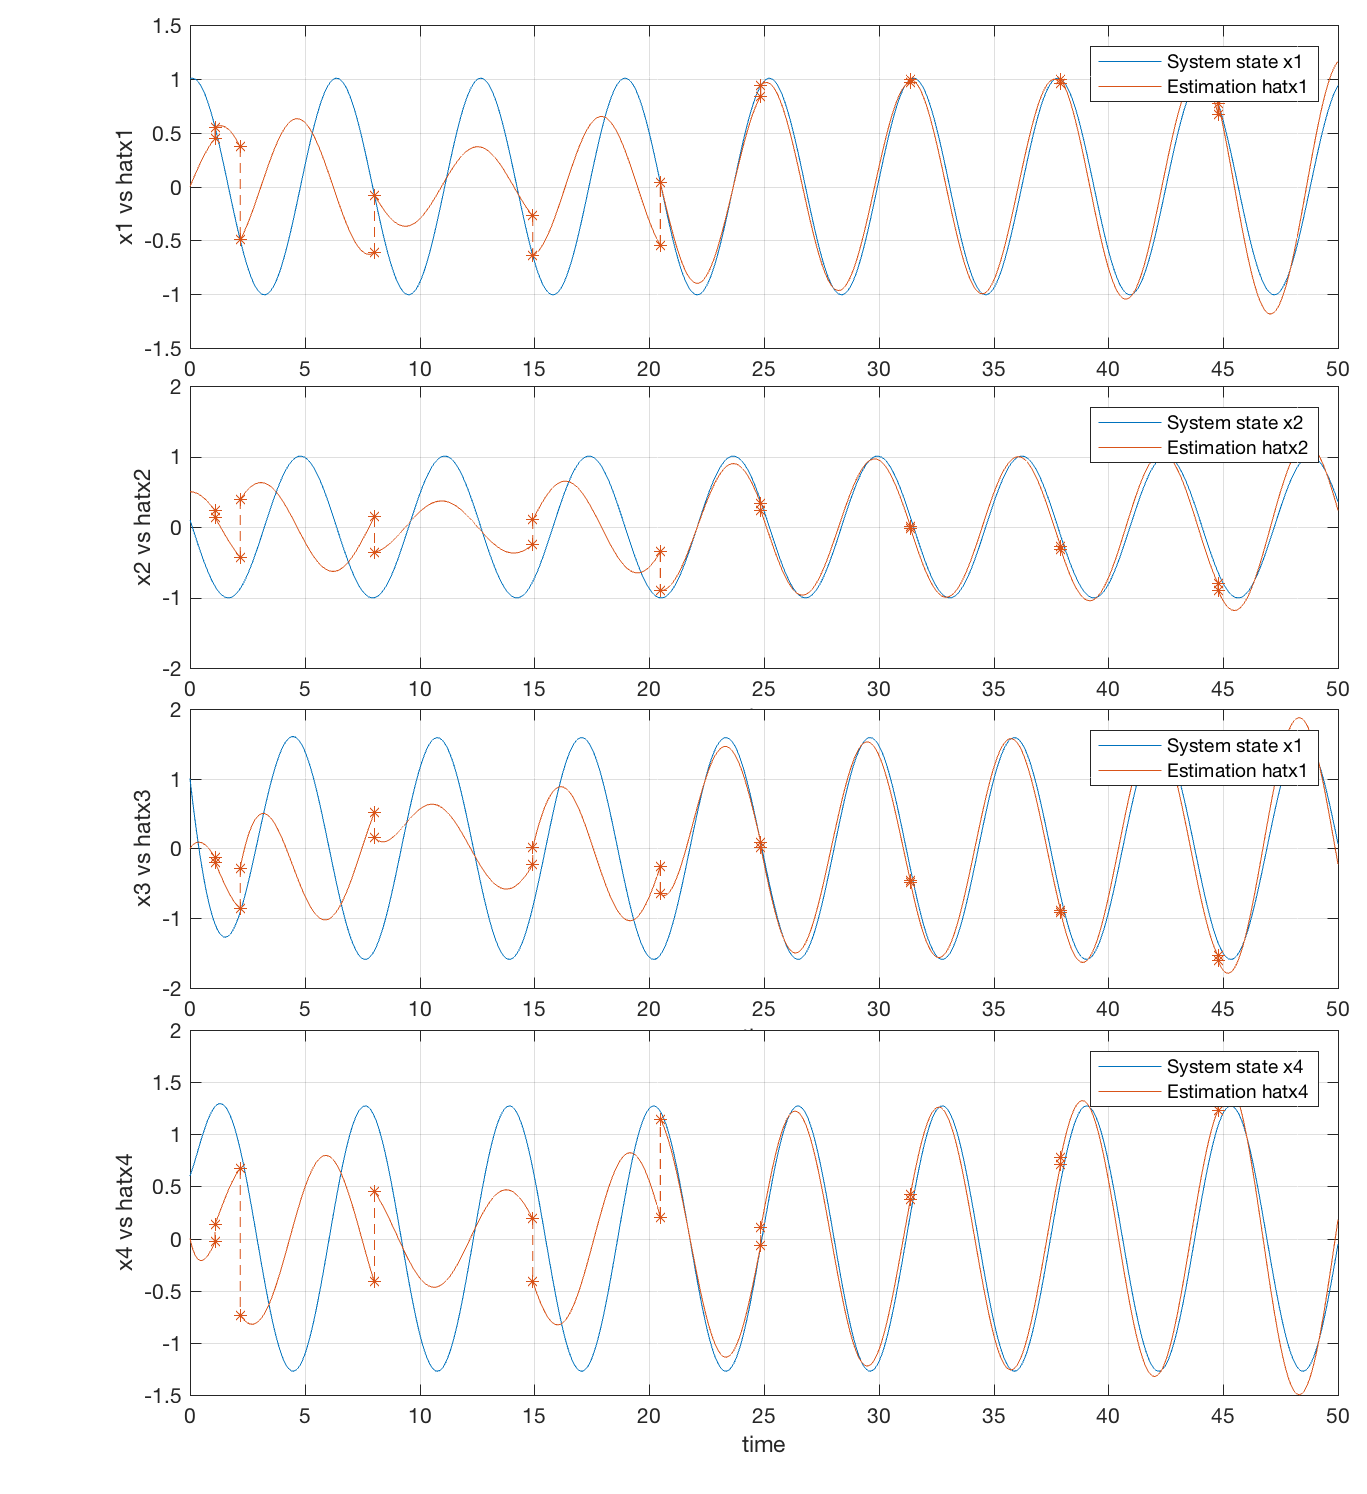
\includegraphics[width=0.8\textwidth]{figures/Simulink/ResultsNetworkEstimator1.eps}
   \caption{Estimated states Vs. continuous plant states}
\label{fig:Net-Est}
  \end{center}
\end{figure}


\begin{itemize}
\item Continuous process:

Flow map
%\scriptsize
% This file was automatically created from the m-file 
% "m2tex.m" written by USL. 
% The fontencoding in this file is UTF-8. 
%  
% You will need to include the following two packages in 
% your LaTeX-Main-File. 
%  
% \usepackage{color} 
% \usepackage{fancyvrb} 
%  
% It is advised to use the following option for Inputenc 
% \usepackage[utf8]{inputenc} 
%  
  
% definition of matlab colors: 
\definecolor{mblue}{rgb}{0,0,1} 
\definecolor{mgreen}{rgb}{0.13333,0.5451,0.13333} 
\definecolor{mred}{rgb}{0.62745,0.12549,0.94118} 
\definecolor{mgrey}{rgb}{0.5,0.5,0.5} 
\definecolor{mdarkgrey}{rgb}{0.25,0.25,0.25} 
  
\DefineShortVerb[fontfamily=courier,fontseries=m]{\$} 
\DefineShortVerb[fontfamily=courier,fontseries=b]{\#} 
  
\noindent                    
 \hspace*{-1.6em}{\scriptsize 1}$  $\color{mblue}$function$\color{black}$ xdot = f(x, u, gamma)$\\
 \hspace*{-1.6em}{\scriptsize 2}$  $\\
 \hspace*{-1.6em}{\scriptsize 3}$  $\color{mgreen}#%%%%%%%%%%%%%%%%%%%%%%%%%%%%%%%%%%%%%%%%%%%%%%%%%%%%%%%%%%%%%%%%%%%%%%%%%%%#\color{black}$$\\
 \hspace*{-1.6em}{\scriptsize 4}$  $\color{mgreen}$% Matlab Function  Author: Ricardo Sanfelice $\color{black}$$\\
 \hspace*{-1.6em}{\scriptsize 5}$  $\color{mgreen}$% (Revised by Giampiero Campa)$\color{black}$$\\
 \hspace*{-1.6em}{\scriptsize 6}$  $\color{mgreen}$% (Revised by Pablo Nanez)$\color{black}$$\\
 \hspace*{-1.6em}{\scriptsize 7}$  $\color{mgreen}$%$\color{black}$$\\
 \hspace*{-1.6em}{\scriptsize 8}$  $\color{mgreen}$% Project: Simulation of a hybrid system (Bouncing Ball)$\color{black}$$\\
 \hspace*{-1.6em}{\scriptsize 9}$  $\color{mgreen}$%$\color{black}$$\\
 \hspace*{-2em}{\scriptsize 10}$  $\color{mgreen}$% Name: f.m$\color{black}$$\\
 \hspace*{-2em}{\scriptsize 11}$  $\color{mgreen}$%$\color{black}$$\\
 \hspace*{-2em}{\scriptsize 12}$  $\color{mgreen}$% Description: Flow map$\color{black}$$\\
 \hspace*{-2em}{\scriptsize 13}$  $\color{mgreen}$%$\color{black}$$\\
 \hspace*{-2em}{\scriptsize 14}$  $\color{mgreen}$% Version: 1.0$\color{black}$$\\
 \hspace*{-2em}{\scriptsize 15}$  $\color{mgreen}$% Required files: - $\color{black}$$\\
 \hspace*{-2em}{\scriptsize 16}$  $\color{mgreen}#%%%%%%%%%%%%%%%%%%%%%%%%%%%%%%%%%%%%%%%%%%%%%%%%%%%%%%%%%%%%%%%%%%%%%%%%%%%#\color{black}$$\\
 \hspace*{-2em}{\scriptsize 17}$  $\\
 \hspace*{-2em}{\scriptsize 18}$  $\\
 \hspace*{-2em}{\scriptsize 19}$  $\color{mgreen}$% flow map: xdot=f(x,u);$\color{black}$$\\
 \hspace*{-2em}{\scriptsize 20}$  xdot = [x(2); gamma];$\\ 
  
\UndefineShortVerb{\$} 
\UndefineShortVerb{\#}\label{scr:f}
%\normalsize

Flow set
%\scriptsize
% This file was automatically created from the m-file 
% "m2tex.m" written by USL. 
% The fontencoding in this file is UTF-8. 
%  
% You will need to include the following two packages in 
% your LaTeX-Main-File. 
%  
% \usepackage{color} 
% \usepackage{fancyvrb} 
%  
% It is advised to use the following option for Inputenc 
% \usepackage[utf8]{inputenc} 
%  
  
% definition of matlab colors: 
\definecolor{mblue}{rgb}{0,0,1} 
\definecolor{mgreen}{rgb}{0.13333,0.5451,0.13333} 
\definecolor{mred}{rgb}{0.62745,0.12549,0.94118} 
\definecolor{mgrey}{rgb}{0.5,0.5,0.5} 
\definecolor{mdarkgrey}{rgb}{0.25,0.25,0.25} 
  
\DefineShortVerb[fontfamily=courier,fontseries=m]{\$} 
\DefineShortVerb[fontfamily=courier,fontseries=b]{\#} 
  
\noindent                          
 \hspace*{-1.6em}{\scriptsize 1}$  $\color{mblue}$function$\color{black}$ v  = C(x, u)$\\
 \hspace*{-1.6em}{\scriptsize 2}$  $\color{mgreen}$%--------------------------------------------------------------------------$\color{black}$$\\
 \hspace*{-1.6em}{\scriptsize 3}$  $\color{mgreen}$% Matlab M-file Project: HyEQ Toolbox @  Hybrid Systems Laboratory (HSL),$\color{black}$$\\
 \hspace*{-1.6em}{\scriptsize 4}$  $\color{mgreen}$% https://hybrid.soe.ucsc.edu/software$\color{black}$$\\
 \hspace*{-1.6em}{\scriptsize 5}$  $\color{mgreen}$% http://hybridsimulator.wordpress.com/$\color{black}$$\\
 \hspace*{-1.6em}{\scriptsize 6}$  $\color{mgreen}$%--------------------------------------------------------------------------$\color{black}$$\\
 \hspace*{-1.6em}{\scriptsize 7}$  $\color{mgreen}$% Project: Simulation of a hybrid system$\color{black}$$\\
 \hspace*{-1.6em}{\scriptsize 8}$  $\color{mgreen}$% Description: Flow set$\color{black}$$\\
 \hspace*{-1.6em}{\scriptsize 9}$  $\color{mgreen}$%--------------------------------------------------------------------------$\color{black}$$\\
 \hspace*{-2em}{\scriptsize 10}$  $\color{mgreen}$%--------------------------------------------------------------------------$\color{black}$$\\
 \hspace*{-2em}{\scriptsize 11}$  $\color{mgreen}$%   See also HYEQSOLVER, PLOTARC, PLOTARC3, PLOTFLOWS, PLOTHARC,$\color{black}$$\\
 \hspace*{-2em}{\scriptsize 12}$  $\color{mgreen}$%   PLOTHARCCOLOR, PLOTHARCCOLOR3D, PLOTHYBRIDARC, PLOTJUMPS.$\color{black}$$\\
 \hspace*{-2em}{\scriptsize 13}$  $\color{mgreen}$%   Copyright @ Hybrid Systems Laboratory (HSL),$\color{black}$$\\
 \hspace*{-2em}{\scriptsize 14}$  $\color{mgreen}$%   Revision: 0.0.0.3 Date: 05/20/2015 3:42:00$\color{black}$$\\
 \hspace*{-2em}{\scriptsize 15}$  $\color{mgreen}$%$\color{black}$$\\
 \hspace*{-2em}{\scriptsize 16}$  $\color{mgreen}$% Check on flow conditions$\color{black}$$\\
 \hspace*{-2em}{\scriptsize 17}$  $\color{mgreen}$% E.g.,$\color{black}$$\\
 \hspace*{-2em}{\scriptsize 18}$  $\color{mgreen}$% if (x(1) >= u(1))  % flow condition$\color{black}$$\\
 \hspace*{-2em}{\scriptsize 19}$  $\color{mgreen}$%     v = 1;  % report flow$\color{black}$$\\
 \hspace*{-2em}{\scriptsize 20}$  $\color{mgreen}$% else$\color{black}$$\\
 \hspace*{-2em}{\scriptsize 21}$  $\color{mgreen}$%     v = 0;   % do not report flow$\color{black}$$\\
 \hspace*{-2em}{\scriptsize 22}$  $\color{mgreen}$% end$\color{black}$$\\
 \hspace*{-2em}{\scriptsize 23}$  $\\
 \hspace*{-2em}{\scriptsize 24}$  $\\
 \hspace*{-2em}{\scriptsize 25}$  v = 1; $\color{mgreen}$% report flow$\color{black}$$\\
 \hspace*{-2em}{\scriptsize 26}$  $\\ 
  
\UndefineShortVerb{\$} 
\UndefineShortVerb{\#}\label{scr:C}
%\normalsize

Jump map
%\scriptsize
% This file was automatically created from the m-file 
% "m2tex.m" written by USL. 
% The fontencoding in this file is UTF-8. 
%  
% You will need to include the following two packages in 
% your LaTeX-Main-File. 
%  
% \usepackage{color} 
% \usepackage{fancyvrb} 
%  
% It is advised to use the following option for Inputenc 
% \usepackage[utf8]{inputenc} 
%  
  
% definition of matlab colors: 
\definecolor{mblue}{rgb}{0,0,1} 
\definecolor{mgreen}{rgb}{0.13333,0.5451,0.13333} 
\definecolor{mred}{rgb}{0.62745,0.12549,0.94118} 
\definecolor{mgrey}{rgb}{0.5,0.5,0.5} 
\definecolor{mdarkgrey}{rgb}{0.25,0.25,0.25} 
  
\DefineShortVerb[fontfamily=courier,fontseries=m]{\$} 
\DefineShortVerb[fontfamily=courier,fontseries=b]{\#} 
  
\noindent   
 \hspace*{-1.6em}{\scriptsize 1}$  $\color{mblue}$function$\color{black}$ xplus = g(x, u, lambda)$\\
 \hspace*{-1.6em}{\scriptsize 2}$  $\color{mgreen}$% jump map$\color{black}$$\\
 \hspace*{-1.6em}{\scriptsize 3}$  xplus = [u(1); -lambda*x(2)];$\\ 
  
\UndefineShortVerb{\$} 
\UndefineShortVerb{\#}\label{scr:g}
%\normalsize

Jump set
%\scriptsize
% This file was automatically created from the m-file 
% "m2tex.m" written by USL. 
% The fontencoding in this file is UTF-8. 
%  
% You will need to include the following two packages in 
% your LaTeX-Main-File. 
%  
% \usepackage{color} 
% \usepackage{fancyvrb} 
%  
% It is advised to use the following option for Inputenc 
% \usepackage[utf8]{inputenc} 
%  
  
% definition of matlab colors: 
\definecolor{mblue}{rgb}{0,0,1} 
\definecolor{mgreen}{rgb}{0.13333,0.5451,0.13333} 
\definecolor{mred}{rgb}{0.62745,0.12549,0.94118} 
\definecolor{mgrey}{rgb}{0.5,0.5,0.5} 
\definecolor{mdarkgrey}{rgb}{0.25,0.25,0.25} 
  
\DefineShortVerb[fontfamily=courier,fontseries=m]{\$} 
\DefineShortVerb[fontfamily=courier,fontseries=b]{\#} 
  
\noindent                         
 \hspace*{-1.6em}{\scriptsize 1}$  $\color{mblue}$function$\color{black}$ v  = D(x, u) $\\
 \hspace*{-1.6em}{\scriptsize 2}$  $\\
 \hspace*{-1.6em}{\scriptsize 3}$  $\color{mgreen}#%%%%%%%%%%%%%%%%%%%%%%%%%%%%%%%%%%%%%%%%%%%%%%%%%%%%%%%%%%%%%%%%%%%%%%%%%%%#\color{black}$$\\
 \hspace*{-1.6em}{\scriptsize 4}$  $\color{mgreen}$% Matlab Function  Author: Ricardo Sanfelice $\color{black}$$\\
 \hspace*{-1.6em}{\scriptsize 5}$  $\color{mgreen}$% (Revised by Giampiero Campa)$\color{black}$$\\
 \hspace*{-1.6em}{\scriptsize 6}$  $\color{mgreen}$% (Revised by Pablo Nanez)$\color{black}$$\\
 \hspace*{-1.6em}{\scriptsize 7}$  $\color{mgreen}$%$\color{black}$$\\
 \hspace*{-1.6em}{\scriptsize 8}$  $\color{mgreen}$% Project: Simulation of a hybrid system (Bouncing ball)$\color{black}$$\\
 \hspace*{-1.6em}{\scriptsize 9}$  $\color{mgreen}$%$\color{black}$$\\
 \hspace*{-2em}{\scriptsize 10}$  $\color{mgreen}$% Name: D.m$\color{black}$$\\
 \hspace*{-2em}{\scriptsize 11}$  $\color{mgreen}$%$\color{black}$$\\
 \hspace*{-2em}{\scriptsize 12}$  $\color{mgreen}$% Description: Jump set$\color{black}$$\\
 \hspace*{-2em}{\scriptsize 13}$  $\color{mgreen}$%$\color{black}$$\\
 \hspace*{-2em}{\scriptsize 14}$  $\color{mgreen}$% Version: 1.0$\color{black}$$\\
 \hspace*{-2em}{\scriptsize 15}$  $\color{mgreen}$% Required files: - $\color{black}$$\\
 \hspace*{-2em}{\scriptsize 16}$  $\color{mgreen}#%%%%%%%%%%%%%%%%%%%%%%%%%%%%%%%%%%%%%%%%%%%%%%%%%%%%%%%%%%%%%%%%%%%%%%%%%%%#\color{black}$$\\
 \hspace*{-2em}{\scriptsize 17}$  $\\
 \hspace*{-2em}{\scriptsize 18}$  xtemp = zeros(2,1);$\\
 \hspace*{-2em}{\scriptsize 19}$  xtemp = x;$\\
 \hspace*{-2em}{\scriptsize 20}$  $\\
 \hspace*{-2em}{\scriptsize 21}$  $\color{mblue}$if$\color{black}$ (xtemp(1) <= u(1)) && (xtemp(2) <= 0)  $\color{mgreen}$% jump condition$\color{black}$$\\
 \hspace*{-2em}{\scriptsize 22}$      v = 1;  $\color{mgreen}$% report jump$\color{black}$$\\
 \hspace*{-2em}{\scriptsize 23}$  $\color{mblue}$else$\color{black}$$\\
 \hspace*{-2em}{\scriptsize 24}$      v = 0;   $\color{mgreen}$% do not report jump$\color{black}$$\\
 \hspace*{-2em}{\scriptsize 25}$  $\color{mblue}$end$\color{black}$$\\ 
  
\UndefineShortVerb{\$} 
\UndefineShortVerb{\#}\label{scr:D}
%\normalsize

\item Network:

Flow map
%\scriptsize
% This file was automatically created from the m-file 
% "m2tex.m" written by USL. 
% The fontencoding in this file is UTF-8. 
%  
% You will need to include the following two packages in 
% your LaTeX-Main-File. 
%  
% \usepackage{color} 
% \usepackage{fancyvrb} 
%  
% It is advised to use the following option for Inputenc 
% \usepackage[utf8]{inputenc} 
%  
  
% definition of matlab colors: 
\definecolor{mblue}{rgb}{0,0,1} 
\definecolor{mgreen}{rgb}{0.13333,0.5451,0.13333} 
\definecolor{mred}{rgb}{0.62745,0.12549,0.94118} 
\definecolor{mgrey}{rgb}{0.5,0.5,0.5} 
\definecolor{mdarkgrey}{rgb}{0.25,0.25,0.25} 
  
\DefineShortVerb[fontfamily=courier,fontseries=m]{\$} 
\DefineShortVerb[fontfamily=courier,fontseries=b]{\#} 
  
\begin{Verbatim}[commandchars=\$\{\},numbers=left,numbersep=2pt] 

    $textcolor{mblue}{function} xdot = f(x,vs) 
    $textcolor{mgreen}{%--------------------------------------------------------------------------} 
    $textcolor{mgreen}{% Matlab M-file Project: HyEQ Toolbox @  Hybrid Systems Laboratory (HSL), } 
    $textcolor{mgreen}{% https://hybrid.soe.ucsc.edu/software} 
    $textcolor{mgreen}{% http://hybridsimulator.wordpress.com/} 
    $textcolor{mgreen}{%--------------------------------------------------------------------------} 
    $textcolor{mgreen}{% Project: Simulation of a hybrid system Digital network (net) } 
    $textcolor{mgreen}{% Description: Flow map} 
    $textcolor{mgreen}{%--------------------------------------------------------------------------} 
    $textcolor{mgreen}{%--------------------------------------------------------------------------} 
    $textcolor{mgreen}{%   See also HYEQSOLVER, PLOTARC, PLOTARC3, PLOTFLOWS, PLOTHARC,} 
    $textcolor{mgreen}{%   PLOTHARCCOLOR, PLOTHARCCOLOR3D, PLOTHYBRIDARC, PLOTJUMPS.} 
    $textcolor{mgreen}{%   Copyright @ Hybrid Systems Laboratory (HSL),} 
    $textcolor{mgreen}{%   Revision: 0.0.0.3 Date: 05/20/2015 3:42:00} 
     
    n = length(vs); $textcolor{mgreen}{% measured input size} 
     
    msdot = zeros(n,1); $textcolor{mgreen}{% measured continuous dynamics} 
    jdot = 0; 
    tau_sdot = -1; $textcolor{mgreen}{% Timer tau_s} 
    xdot = [msdot;jdot;tau_sdot]; 
      
\end{Verbatim}  
  
\UndefineShortVerb{\$} 
\UndefineShortVerb{\#} 
 \label{scr:f}
%\normalsize

Flow set
%\scriptsize
% This file was automatically created from the m-file 
% "m2tex.m" written by USL. 
% The fontencoding in this file is UTF-8. 
%  
% You will need to include the following two packages in 
% your LaTeX-Main-File. 
%  
% \usepackage{color} 
% \usepackage{fancyvrb} 
%  
% It is advised to use the following option for Inputenc 
% \usepackage[utf8]{inputenc} 
%  
  
% definition of matlab colors: 
\definecolor{mblue}{rgb}{0,0,1} 
\definecolor{mgreen}{rgb}{0.13333,0.5451,0.13333} 
\definecolor{mred}{rgb}{0.62745,0.12549,0.94118} 
\definecolor{mgrey}{rgb}{0.5,0.5,0.5} 
\definecolor{mdarkgrey}{rgb}{0.25,0.25,0.25} 
  
\DefineShortVerb[fontfamily=courier,fontseries=m]{\$} 
\DefineShortVerb[fontfamily=courier,fontseries=b]{\#} 
  
\begin{Verbatim}[commandchars=\$\{\},numbers=left,numbersep=2pt] 

    $textcolor{mblue}{function} v  = C(x, vs, Tnmax)  
    $textcolor{mgreen}{%--------------------------------------------------------------------------} 
    $textcolor{mgreen}{% Matlab M-file Project: HyEQ Toolbox @  Hybrid Systems Laboratory (HSL), } 
    $textcolor{mgreen}{% https://hybrid.soe.ucsc.edu/software} 
    $textcolor{mgreen}{% http://hybridsimulator.wordpress.com/} 
    $textcolor{mgreen}{%--------------------------------------------------------------------------} 
    $textcolor{mgreen}{% Project: Simulation of a hybrid system Digital network (net) } 
    $textcolor{mgreen}{% Description: Flow set} 
    $textcolor{mgreen}{%--------------------------------------------------------------------------} 
    $textcolor{mgreen}{%--------------------------------------------------------------------------} 
    $textcolor{mgreen}{%   See also HYEQSOLVER, PLOTARC, PLOTARC3, PLOTFLOWS, PLOTHARC,} 
    $textcolor{mgreen}{%   PLOTHARCCOLOR, PLOTHARCCOLOR3D, PLOTHYBRIDARC, PLOTJUMPS.} 
    $textcolor{mgreen}{%   Copyright @ Hybrid Systems Laboratory (HSL),} 
    $textcolor{mgreen} 
    $textcolor{mgreen}{% Check on flow conditions} 
    $textcolor{mgreen}{% E.g.,} 
    $textcolor{mgreen}{% if (x(1) >= u(1))  % flow condition} 
    $textcolor{mgreen}{%     v = 1;  % report flow} 
    $textcolor{mgreen}{% else} 
    $textcolor{mgreen}{%     v = 0;   % do not report flow} 
    $textcolor{mgreen}{% end} 
     
    tau_s = x(end); $textcolor{mgreen}{% timer state} 
     
    $textcolor{mblue}{if} tau_s>=0 && tau_s<= Tnmax 
        v = 1; $textcolor{mgreen}{% report flow} 
    $textcolor{mblue}{elseif} tau_s> Tnmax 
        v = 0; $textcolor{mgreen}{% do not report flow} 
    $textcolor{mblue}{else} 
        v = 0; 
    $textcolor{mblue}{end}  
\end{Verbatim}  
  
\UndefineShortVerb{\$} 
\UndefineShortVerb{\#} 
 \label{scr:C}
%\normalsize

Jump map
%\scriptsize
% This file was automatically created from the m-file 
% "m2tex.m" written by USL. 
% The fontencoding in this file is UTF-8. 
%  
% You will need to include the following two packages in 
% your LaTeX-Main-File. 
%  
% \usepackage{color} 
% \usepackage{fancyvrb} 
%  
% It is advised to use the following option for Inputenc 
% \usepackage[utf8]{inputenc} 
%  
  
% definition of matlab colors: 
\definecolor{mblue}{rgb}{0,0,1} 
\definecolor{mgreen}{rgb}{0.13333,0.5451,0.13333} 
\definecolor{mred}{rgb}{0.62745,0.12549,0.94118} 
\definecolor{mgrey}{rgb}{0.5,0.5,0.5} 
\definecolor{mdarkgrey}{rgb}{0.25,0.25,0.25} 
  
\DefineShortVerb[fontfamily=courier,fontseries=m]{\$} 
\DefineShortVerb[fontfamily=courier,fontseries=b]{\#} 
  
\noindent                              
 \hspace*{-1.6em}{\scriptsize 1}$  $\color{mblue}$function$\color{black}$ xplus = g(x, vs, Tnmax, Tnmin, tk)$\\
 \hspace*{-1.6em}{\scriptsize 2}$  $\color{mgreen}$%--------------------------------------------------------------------------$\color{black}$$\\
 \hspace*{-1.6em}{\scriptsize 3}$  $\color{mgreen}$% Matlab M-file Project: HyEQ Toolbox @  Hybrid Systems Laboratory (HSL), $\color{black}$$\\
 \hspace*{-1.6em}{\scriptsize 4}$  $\color{mgreen}$% https://hybrid.soe.ucsc.edu/software$\color{black}$$\\
 \hspace*{-1.6em}{\scriptsize 5}$  $\color{mgreen}$% http://hybridsimulator.wordpress.com/$\color{black}$$\\
 \hspace*{-1.6em}{\scriptsize 6}$  $\color{mgreen}$%--------------------------------------------------------------------------$\color{black}$$\\
 \hspace*{-1.6em}{\scriptsize 7}$  $\color{mgreen}$% Project: Simulation of a hybrid system Analog-to-Digital converter (ADC) $\color{black}$$\\
 \hspace*{-1.6em}{\scriptsize 8}$  $\color{mgreen}$% Description: Jump map$\color{black}$$\\
 \hspace*{-1.6em}{\scriptsize 9}$  $\color{mgreen}$%--------------------------------------------------------------------------$\color{black}$$\\
 \hspace*{-2em}{\scriptsize 10}$  $\color{mgreen}$%--------------------------------------------------------------------------$\color{black}$$\\
 \hspace*{-2em}{\scriptsize 11}$  $\color{mgreen}$%   See also HYEQSOLVER, PLOTARC, PLOTARC3, PLOTFLOWS, PLOTHARC,$\color{black}$$\\
 \hspace*{-2em}{\scriptsize 12}$  $\color{mgreen}$%   PLOTHARCCOLOR, PLOTHARCCOLOR3D, PLOTHYBRIDARC, PLOTJUMPS.$\color{black}$$\\
 \hspace*{-2em}{\scriptsize 13}$  $\color{mgreen}$%   Copyright @ Hybrid Systems Laboratory (HSL),$\color{black}$$\\
 \hspace*{-2em}{\scriptsize 14}$  $\color{mgreen}$%   Revision: 0.0.0.3 Date: 05/20/2015 3:42:00$\color{black}$$\\
 \hspace*{-2em}{\scriptsize 15}$  $\\
 \hspace*{-2em}{\scriptsize 16}$  n = length(vs); $\color{mgreen}$% measured input size$\color{black}$$\\
 \hspace*{-2em}{\scriptsize 17}$  xtemp = zeros(n+2,1);$\\
 \hspace*{-2em}{\scriptsize 18}$  xtemp = x;$\\
 \hspace*{-2em}{\scriptsize 19}$  x = xtemp;$\\
 \hspace*{-2em}{\scriptsize 20}$  $\\
 \hspace*{-2em}{\scriptsize 21}$  $\\
 \hspace*{-2em}{\scriptsize 22}$  j = x(n+1);$\\
 \hspace*{-2em}{\scriptsize 23}$  msplus = vs; $\color{mgreen}$% output = measured input$\color{black}$$\\
 \hspace*{-2em}{\scriptsize 24}$  $\color{mgreen}$% The value tau_s is updated as a function of vs, e.g., $\color{black}$$\\
 \hspace*{-2em}{\scriptsize 25}$  tau_splus = tk(j+1); $\color{mgreen}$% Timer tau_s$\color{black}$$\\
 \hspace*{-2em}{\scriptsize 26}$  j_plus = j+1;$\\
 \hspace*{-2em}{\scriptsize 27}$  xplus = [msplus;j_plus;tau_splus];$\\
 \hspace*{-2em}{\scriptsize 28}$  $\\
 \hspace*{-2em}{\scriptsize 29}$  $\\
 \hspace*{-2em}{\scriptsize 30}$  $\\ 
  
\UndefineShortVerb{\$} 
\UndefineShortVerb{\#}\label{scr:g}
%\normalsize

Jump set
%\scriptsize
% This file was automatically created from the m-file 
% "m2tex.m" written by USL. 
% The fontencoding in this file is UTF-8. 
%  
% You will need to include the following two packages in 
% your LaTeX-Main-File. 
%  
% \usepackage{color} 
% \usepackage{fancyvrb} 
%  
% It is advised to use the following option for Inputenc 
% \usepackage[utf8]{inputenc} 
%  
  
% definition of matlab colors: 
\definecolor{mblue}{rgb}{0,0,1} 
\definecolor{mgreen}{rgb}{0.13333,0.5451,0.13333} 
\definecolor{mred}{rgb}{0.62745,0.12549,0.94118} 
\definecolor{mgrey}{rgb}{0.5,0.5,0.5} 
\definecolor{mdarkgrey}{rgb}{0.25,0.25,0.25} 
  
\DefineShortVerb[fontfamily=courier,fontseries=m]{\$} 
\DefineShortVerb[fontfamily=courier,fontseries=b]{\#} 
  
\begin{Verbatim}[commandchars=\$\{\},numbers=left,numbersep=2pt] 

    $textcolor{mblue}{function} v  = D(x, vs)  
    $textcolor{mgreen}{%--------------------------------------------------------------------------} 
    $textcolor{mgreen}{% Matlab M-file Project: HyEQ Toolbox @  Hybrid Systems Laboratory (HSL), } 
    $textcolor{mgreen}{% https://hybrid.soe.ucsc.edu/software} 
    $textcolor{mgreen}{% http://hybridsimulator.wordpress.com/} 
    $textcolor{mgreen}{%--------------------------------------------------------------------------} 
    $textcolor{mgreen}{% Project: Simulation of a hybrid system Analog-to-Digital converter (ADC) } 
    $textcolor{mgreen}{% Description: Jump set} 
    $textcolor{mgreen}{%--------------------------------------------------------------------------} 
    $textcolor{mgreen}{%--------------------------------------------------------------------------} 
    $textcolor{mgreen}{%   See also HYEQSOLVER, PLOTARC, PLOTARC3, PLOTFLOWS, PLOTHARC,} 
    $textcolor{mgreen}{%   PLOTHARCCOLOR, PLOTHARCCOLOR3D, PLOTHYBRIDARC, PLOTJUMPS.} 
    $textcolor{mgreen}{%   Copyright @ Hybrid Systems Laboratory (HSL),} 
    $textcolor{mgreen} 
    $textcolor{mgreen}{% Check on jump conditions} 
    $textcolor{mgreen}{% % E.g.,} 
    $textcolor{mgreen}{% if (x(1) <= u(1)) && (x(2) <= 0)  % jump condition} 
    $textcolor{mgreen}{%     v = 1;  % report jump} 
    $textcolor{mgreen}{% else} 
    $textcolor{mgreen}{%     v = 0;   % do not report jump} 
    $textcolor{mgreen}{% end} 
     
     
    tau_s = x(end); $textcolor{mgreen}{% timer state} 
     
    $textcolor{mblue}{if} tau_s>=0 
        v = 0; $textcolor{mgreen}{% do not report jump} 
    $textcolor{mblue}{elseif} tau_s<= 0 
        v = 1; $textcolor{mgreen}{% report jump} 
    $textcolor{mblue}{else} 
        v = 0; 
    $textcolor{mblue}{end}  
\end{Verbatim}  
  
\UndefineShortVerb{\$} 
\UndefineShortVerb{\#} 
 \label{scr:D}
%\normalsize

\item Estimator:

Flow map
%\scriptsize
% This file was automatically created from the m-file 
% "m2tex.m" written by USL. 
% The fontencoding in this file is UTF-8. 
%  
% You will need to include the following two packages in 
% your LaTeX-Main-File. 
%  
% \usepackage{color} 
% \usepackage{fancyvrb} 
%  
% It is advised to use the following option for Inputenc 
% \usepackage[utf8]{inputenc} 
%  
  
% definition of matlab colors: 
\definecolor{mblue}{rgb}{0,0,1} 
\definecolor{mgreen}{rgb}{0.13333,0.5451,0.13333} 
\definecolor{mred}{rgb}{0.62745,0.12549,0.94118} 
\definecolor{mgrey}{rgb}{0.5,0.5,0.5} 
\definecolor{mdarkgrey}{rgb}{0.25,0.25,0.25} 
  
\DefineShortVerb[fontfamily=courier,fontseries=m]{\$} 
\DefineShortVerb[fontfamily=courier,fontseries=b]{\#} 
  
\begin{Verbatim}[commandchars=\$\{\},numbers=left,numbersep=2pt] 

    $textcolor{mblue}{function} xdot = f(x, v,ctes) 
    $textcolor{mgreen}{%--------------------------------------------------------------------------} 
    $textcolor{mgreen}{% Matlab M-file Project: HyEQ Toolbox @  Hybrid Systems Laboratory (HSL), } 
    $textcolor{mgreen}{% https://hybrid.soe.ucsc.edu/software} 
    $textcolor{mgreen}{% http://hybridsimulator.wordpress.com/} 
    $textcolor{mgreen}{%--------------------------------------------------------------------------} 
    $textcolor{mgreen}{% Project: Simulation of a hybrid system} 
    $textcolor{mgreen}{% Description: Flow map} 
    $textcolor{mgreen}{%--------------------------------------------------------------------------} 
    $textcolor{mgreen}{%--------------------------------------------------------------------------} 
    $textcolor{mgreen}{%   See also HYEQSOLVER, PLOTARC, PLOTARC3, PLOTFLOWS, PLOTHARC,} 
    $textcolor{mgreen}{%   PLOTHARCCOLOR, PLOTHARCCOLOR3D, PLOTHYBRIDARC, PLOTJUMPS.} 
    $textcolor{mgreen}{%   Copyright @ Hybrid Systems Laboratory (HSL),} 
    $textcolor{mgreen}{%   Revision: 0.0.0.3 Date: 05/20/2015 3:42:00} 
    $textcolor{mgreen}{%--------------------------------------------------------------------------} 
    $textcolor{mgreen}{% flow map: xdot=f(x,u);} 
    $textcolor{mgreen}{% ctes = [A,B,M',L,P];} 
     
    A = ctes(:,1:4); 
    B = ctes(:,5); 
    $textcolor{mgreen}{% M = ctes(:,6)';} 
    $textcolor{mgreen}{% L = ctes(:,7);} 
    n = length(A); 
    u = v(end); 
    z = x(1:n); 
    jdot = 0; 
    zdot = A*z + B*u; 
    xdot = [zdot;jdot];  
\end{Verbatim}  
  
\UndefineShortVerb{\$} 
\UndefineShortVerb{\#} 
 \label{scr:f}
%\normalsize

Flow set
%\scriptsize
% This file was automatically created from the m-file 
% "m2tex.m" written by USL. 
% The fontencoding in this file is UTF-8. 
%  
% You will need to include the following two packages in 
% your LaTeX-Main-File. 
%  
% \usepackage{color} 
% \usepackage{fancyvrb} 
%  
% It is advised to use the following option for Inputenc 
% \usepackage[utf8]{inputenc} 
%  
  
% definition of matlab colors: 
\definecolor{mblue}{rgb}{0,0,1} 
\definecolor{mgreen}{rgb}{0.13333,0.5451,0.13333} 
\definecolor{mred}{rgb}{0.62745,0.12549,0.94118} 
\definecolor{mgrey}{rgb}{0.5,0.5,0.5} 
\definecolor{mdarkgrey}{rgb}{0.25,0.25,0.25} 
  
\DefineShortVerb[fontfamily=courier,fontseries=m]{\$} 
\DefineShortVerb[fontfamily=courier,fontseries=b]{\#} 
  
\noindent                               
 \hspace*{-1.6em}{\scriptsize 1}$  $\color{mblue}$function$\color{black}$ out  = C(x, v) $\\
 \hspace*{-1.6em}{\scriptsize 2}$  $\color{mgreen}$%--------------------------------------------------------------------------$\color{black}$$\\
 \hspace*{-1.6em}{\scriptsize 3}$  $\color{mgreen}$% Matlab M-file Project: HyEQ Toolbox @  Hybrid Systems Laboratory (HSL), $\color{black}$$\\
 \hspace*{-1.6em}{\scriptsize 4}$  $\color{mgreen}$% https://hybrid.soe.ucsc.edu/software$\color{black}$$\\
 \hspace*{-1.6em}{\scriptsize 5}$  $\color{mgreen}$% http://hybridsimulator.wordpress.com/$\color{black}$$\\
 \hspace*{-1.6em}{\scriptsize 6}$  $\color{mgreen}$%--------------------------------------------------------------------------$\color{black}$$\\
 \hspace*{-1.6em}{\scriptsize 7}$  $\color{mgreen}$% Project: Simulation of a hybrid system$\color{black}$$\\
 \hspace*{-1.6em}{\scriptsize 8}$  $\color{mgreen}$% Description: Flow set$\color{black}$$\\
 \hspace*{-1.6em}{\scriptsize 9}$  $\color{mgreen}$%--------------------------------------------------------------------------$\color{black}$$\\
 \hspace*{-2em}{\scriptsize 10}$  $\color{mgreen}$%--------------------------------------------------------------------------$\color{black}$$\\
 \hspace*{-2em}{\scriptsize 11}$  $\color{mgreen}$%   See also HYEQSOLVER, PLOTARC, PLOTARC3, PLOTFLOWS, PLOTHARC,$\color{black}$$\\
 \hspace*{-2em}{\scriptsize 12}$  $\color{mgreen}$%   PLOTHARCCOLOR, PLOTHARCCOLOR3D, PLOTHYBRIDARC, PLOTJUMPS.$\color{black}$$\\
 \hspace*{-2em}{\scriptsize 13}$  $\color{mgreen}$%   Copyright @ Hybrid Systems Laboratory (HSL),$\color{black}$$\\
 \hspace*{-2em}{\scriptsize 14}$  $\color{mgreen}$%   Revision: 0.0.0.3 Date: 05/20/2015 3:42:00$\color{black}$$\\
 \hspace*{-2em}{\scriptsize 15}$  $\color{mgreen}$%$\color{black}$$\\
 \hspace*{-2em}{\scriptsize 16}$  $\color{mgreen}$% Check on flow conditions$\color{black}$$\\
 \hspace*{-2em}{\scriptsize 17}$  $\color{mgreen}$% E.g.,$\color{black}$$\\
 \hspace*{-2em}{\scriptsize 18}$  $\color{mgreen}$% if (x(1) >= u(1))  % flow condition$\color{black}$$\\
 \hspace*{-2em}{\scriptsize 19}$  $\color{mgreen}$%     v = 1;  % report flow$\color{black}$$\\
 \hspace*{-2em}{\scriptsize 20}$  $\color{mgreen}$% else$\color{black}$$\\
 \hspace*{-2em}{\scriptsize 21}$  $\color{mgreen}$%     v = 0;   % do not report flow$\color{black}$$\\
 \hspace*{-2em}{\scriptsize 22}$  $\color{mgreen}$% end$\color{black}$$\\
 \hspace*{-2em}{\scriptsize 23}$  $\\
 \hspace*{-2em}{\scriptsize 24}$  j = x(end); $\color{mgreen}$% internal communication memory event$\color{black}$$\\
 \hspace*{-2em}{\scriptsize 25}$  jnet = v(end-2); $\color{mgreen}$% communication event$\color{black}$$\\
 \hspace*{-2em}{\scriptsize 26}$  $\\
 \hspace*{-2em}{\scriptsize 27}$  $\color{mblue}$if$\color{black}$ j == jnet$\\
 \hspace*{-2em}{\scriptsize 28}$      out = 1; $\color{mgreen}$% report flow$\color{black}$$\\
 \hspace*{-2em}{\scriptsize 29}$  $\color{mblue}$else$\color{black}$$\\
 \hspace*{-2em}{\scriptsize 30}$      out = 0;$\\
 \hspace*{-2em}{\scriptsize 31}$  $\color{mblue}$end$\color{black}$$\\ 
  
\UndefineShortVerb{\$} 
\UndefineShortVerb{\#}\label{scr:C}
%\normalsize

Jump map
%\scriptsize
% This file was automatically created from the m-file 
% "m2tex.m" written by USL. 
% The fontencoding in this file is UTF-8. 
%  
% You will need to include the following two packages in 
% your LaTeX-Main-File. 
%  
% \usepackage{color} 
% \usepackage{fancyvrb} 
%  
% It is advised to use the following option for Inputenc 
% \usepackage[utf8]{inputenc} 
%  
  
% definition of matlab colors: 
\definecolor{mblue}{rgb}{0,0,1} 
\definecolor{mgreen}{rgb}{0.13333,0.5451,0.13333} 
\definecolor{mred}{rgb}{0.62745,0.12549,0.94118} 
\definecolor{mgrey}{rgb}{0.5,0.5,0.5} 
\definecolor{mdarkgrey}{rgb}{0.25,0.25,0.25} 
  
\DefineShortVerb[fontfamily=courier,fontseries=m]{\$} 
\DefineShortVerb[fontfamily=courier,fontseries=b]{\#} 
  
\noindent                                
 \hspace*{-1.6em}{\scriptsize 1}$  $\color{mblue}$function$\color{black}$ xplus = g(x, v, ctes)$\\
 \hspace*{-1.6em}{\scriptsize 2}$  $\color{mgreen}$%--------------------------------------------------------------------------$\color{black}$$\\
 \hspace*{-1.6em}{\scriptsize 3}$  $\color{mgreen}$% Matlab M-file Project: HyEQ Toolbox @  Hybrid Systems Laboratory (HSL), $\color{black}$$\\
 \hspace*{-1.6em}{\scriptsize 4}$  $\color{mgreen}$% https://hybrid.soe.ucsc.edu/software$\color{black}$$\\
 \hspace*{-1.6em}{\scriptsize 5}$  $\color{mgreen}$% http://hybridsimulator.wordpress.com/$\color{black}$$\\
 \hspace*{-1.6em}{\scriptsize 6}$  $\color{mgreen}$%--------------------------------------------------------------------------$\color{black}$$\\
 \hspace*{-1.6em}{\scriptsize 7}$  $\color{mgreen}$% Project: Simulation of a hybrid system$\color{black}$$\\
 \hspace*{-1.6em}{\scriptsize 8}$  $\color{mgreen}$% Description: Jump map$\color{black}$$\\
 \hspace*{-1.6em}{\scriptsize 9}$  $\color{mgreen}$%--------------------------------------------------------------------------$\color{black}$$\\
 \hspace*{-2em}{\scriptsize 10}$  $\color{mgreen}$%--------------------------------------------------------------------------$\color{black}$$\\
 \hspace*{-2em}{\scriptsize 11}$  $\color{mgreen}$%   See also HYEQSOLVER, PLOTARC, PLOTARC3, PLOTFLOWS, PLOTHARC,$\color{black}$$\\
 \hspace*{-2em}{\scriptsize 12}$  $\color{mgreen}$%   PLOTHARCCOLOR, PLOTHARCCOLOR3D, PLOTHYBRIDARC, PLOTJUMPS.$\color{black}$$\\
 \hspace*{-2em}{\scriptsize 13}$  $\color{mgreen}$%   Copyright @ Hybrid Systems Laboratory (HSL),$\color{black}$$\\
 \hspace*{-2em}{\scriptsize 14}$  $\color{mgreen}$%   Revision: 0.0.0.3 Date: 05/20/2015 3:42:00$\color{black}$$\\
 \hspace*{-2em}{\scriptsize 15}$  $\color{mgreen}$%--------------------------------------------------------------------------$\color{black}$$\\
 \hspace*{-2em}{\scriptsize 16}$  $\color{mgreen}$% jump map: xplus = g(x,u);$\color{black}$$\\
 \hspace*{-2em}{\scriptsize 17}$  $\\
 \hspace*{-2em}{\scriptsize 18}$  A = ctes(:,1:4);$\\
 \hspace*{-2em}{\scriptsize 19}$  M = ctes(:,6)';$\\
 \hspace*{-2em}{\scriptsize 20}$  L = ctes(:,7);$\\
 \hspace*{-2em}{\scriptsize 21}$  $\\
 \hspace*{-2em}{\scriptsize 22}$  n = 4;$\\
 \hspace*{-2em}{\scriptsize 23}$  z = zeros(4,1);$\\
 \hspace*{-2em}{\scriptsize 24}$  zplus = zeros(4,1);$\\
 \hspace*{-2em}{\scriptsize 25}$  xplus = zeros(5,1);$\\
 \hspace*{-2em}{\scriptsize 26}$  z = x(1:4);$\\
 \hspace*{-2em}{\scriptsize 27}$  jnet = v(2); $\color{mgreen}$% communication event$\color{black}$$\\
 \hspace*{-2em}{\scriptsize 28}$  y = v(1);$\\
 \hspace*{-2em}{\scriptsize 29}$  $\\
 \hspace*{-2em}{\scriptsize 30}$  jplus = jnet;$\\
 \hspace*{-2em}{\scriptsize 31}$  zplus = z + L*(y-M*z);$\\
 \hspace*{-2em}{\scriptsize 32}$  xplus = [zplus;jplus];$\\ 
  
\UndefineShortVerb{\$} 
\UndefineShortVerb{\#}\label{scr:g}
%\normalsize

Jump set
%\scriptsize
% This file was automatically created from the m-file 
% "m2tex.m" written by USL. 
% The fontencoding in this file is UTF-8. 
%  
% You will need to include the following two packages in 
% your LaTeX-Main-File. 
%  
% \usepackage{color} 
% \usepackage{fancyvrb} 
%  
% It is advised to use the following option for Inputenc 
% \usepackage[utf8]{inputenc} 
%  
  
% definition of matlab colors: 
\definecolor{mblue}{rgb}{0,0,1} 
\definecolor{mgreen}{rgb}{0.13333,0.5451,0.13333} 
\definecolor{mred}{rgb}{0.62745,0.12549,0.94118} 
\definecolor{mgrey}{rgb}{0.5,0.5,0.5} 
\definecolor{mdarkgrey}{rgb}{0.25,0.25,0.25} 
  
\DefineShortVerb[fontfamily=courier,fontseries=m]{\$} 
\DefineShortVerb[fontfamily=courier,fontseries=b]{\#} 
  
\begin{Verbatim}[commandchars=\$\{\},numbers=left,numbersep=2pt] 

    $textcolor{mblue}{function} out  = D(x, v)  
    $textcolor{mgreen}{%--------------------------------------------------------------------------} 
    $textcolor{mgreen}{% Matlab M-file Project: HyEQ Toolbox @  Hybrid Systems Laboratory (HSL), } 
    $textcolor{mgreen}{% https://hybrid.soe.ucsc.edu/software} 
    $textcolor{mgreen}{% http://hybridsimulator.wordpress.com/} 
    $textcolor{mgreen}{%--------------------------------------------------------------------------} 
    $textcolor{mgreen}{% Project: Simulation of a hybrid system} 
    $textcolor{mgreen}{% Description: Jump set} 
    $textcolor{mgreen}{%--------------------------------------------------------------------------} 
    $textcolor{mgreen}{%--------------------------------------------------------------------------} 
    $textcolor{mgreen}{%   See also HYEQSOLVER, PLOTARC, PLOTARC3, PLOTFLOWS, PLOTHARC,} 
    $textcolor{mgreen}{%   PLOTHARCCOLOR, PLOTHARCCOLOR3D, PLOTHYBRIDARC, PLOTJUMPS.} 
    $textcolor{mgreen}{%   Copyright @ Hybrid Systems Laboratory (HSL),} 
    $textcolor{mgreen} 
    $textcolor{mgreen}{% Check on jump conditions} 
    $textcolor{mgreen}{% % E.g.,} 
    $textcolor{mgreen}{% if (x(1) <= u(1)) && (x(2) <= 0)  % jump condition} 
    $textcolor{mgreen}{%     v = 1;  % report jump} 
    $textcolor{mgreen}{% else} 
    $textcolor{mgreen}{%     v = 0;   % do not report jump} 
    $textcolor{mgreen}{% end} 
     
     
    n = length(x)-1; $textcolor{mgreen}{% measured input size} 
    j = x(end); $textcolor{mgreen}{% internal communication memory event} 
    jnet = v(end-2); $textcolor{mgreen}{% communication event} 
     
    $textcolor{mblue}{if} j ~= jnet 
        out = 1; $textcolor{mgreen}{% report jump} 
    $textcolor{mblue}{else} 
        out = 0; 
    $textcolor{mblue}{end} 
      
\end{Verbatim}  
  
\UndefineShortVerb{\$} 
\UndefineShortVerb{\#} 
 \label{scr:D}
%\normalsize
\end{itemize}

\end{example}